\DiaryEntry{Complex Analysis, 3}{2026-03-23}{Complex Analysis}

In this entry we consider mappings between complex functions (in a similar spirit as we considered the mappings induced by the complex exponential in the previous entry).


\subsection{Complex Factor}

The most simple case is multiplication by a complex factor $a$; ie

\bee
w = a \cdot z
\eee

We can see the effect of the mapping more clearly by considering polar coordinates. With $z = r e^{j \theta}$ and  $a = |a| e^{j \alpha}$, we obtain

\bee
w = |a| \cdot z = a r e^{j (\theta + \alpha)}
\eee

Tt follows that the transformation expands or contracts the vector representing $z$ by the factor $|a|$ and rotates it through an angle $\alpha$ about the origin. The image of a given region is therefore geometrically similar to that region. Thus, in particular, a dilation maps a straight line onto a straight line and a circle onto a circle.


\subsection{Linear Mapping}

A bit more complex is the general linear mapping given by

\bee
w = a \cdot z + b
\eee

with $a = |a| e^{j \alpha}$, $b = b_x + j b_y$. This corresponds to a expansion or contraction (easiest represented in polar coordinates) followed by a translation by $b$ (easiest represented in rectangular coordinates).

\subsection{Exponentiation}

\bee
w = z^n
\eee

With $z = r e^{j \theta}$, we obtain $w = r^n e^{j n \theta}$. Below plot shows the effect on lines: Lines on the real and imaginary axis in the $z$-plane are mapped to lines in the $w$-plane; all other lines are mapped to curves.

For example, the curve $x = x, y = t$ gives $z = x + jt \rightarrow w = z^2 = x^2 - t^2 + j 2xt$. This corresponds to $u = x^2 - t^2, v = 2xt$. We can arrange this to $t = v / 2x$ and then we obtain

\bee
u = x^2 - t^2 = x^2 - \frac{v^2}{4x^2}
\eee

which are parabolas. 

\begin{figure}[H]
\centering
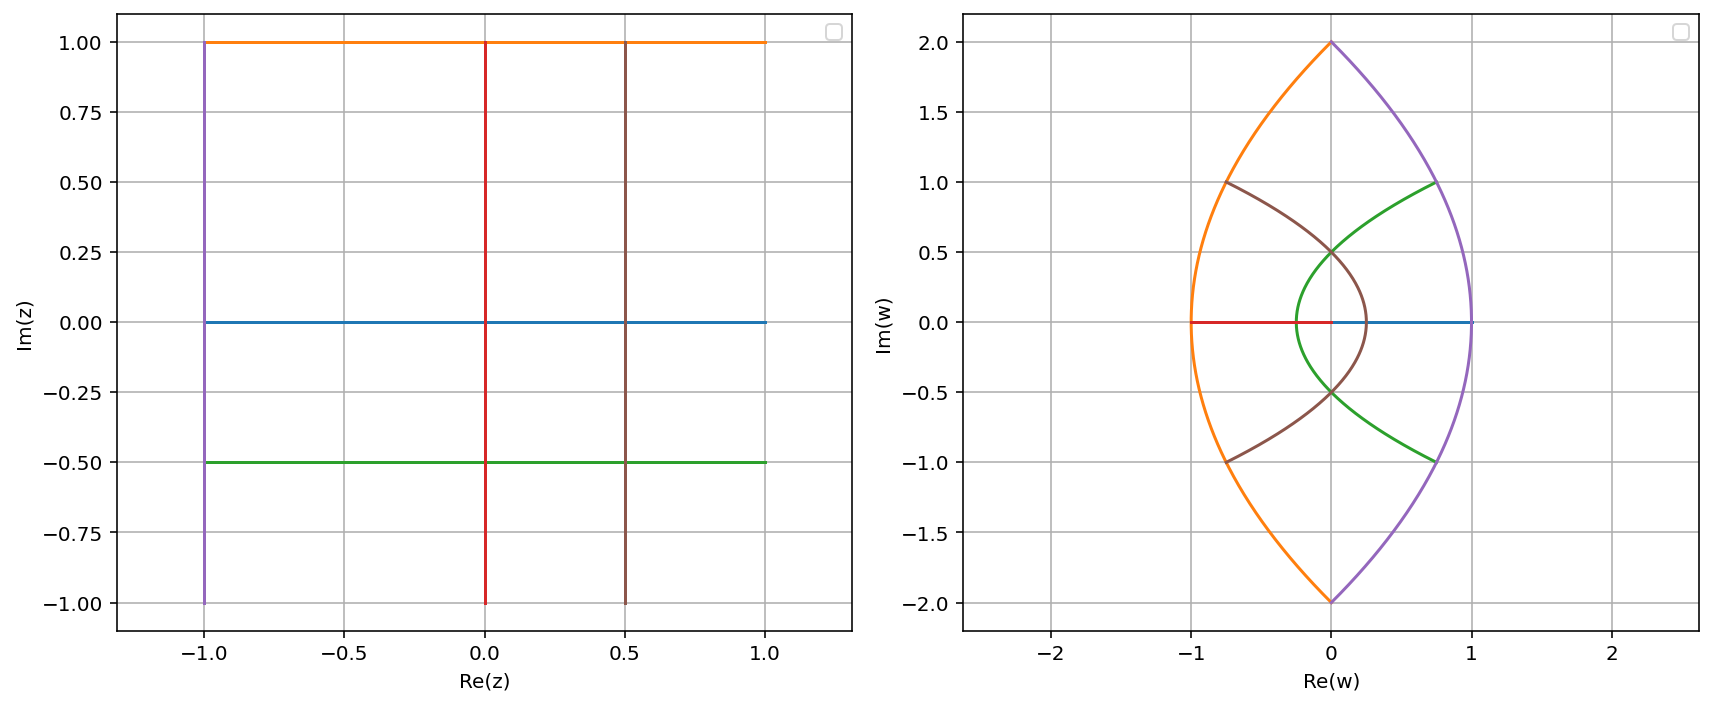
\includegraphics[scale=0.4]{images/2026-03-23-complex_01.png}
\end{figure}

It's also interestng to note that circle stays circles as shown in the plot below. We best see that in the polar expression, $w = r^n e^{j n \theta}$: The radius changes and the circle is traversed two times (so a half-circle becomes a full circle as shown below).

\begin{figure}[H]
\centering
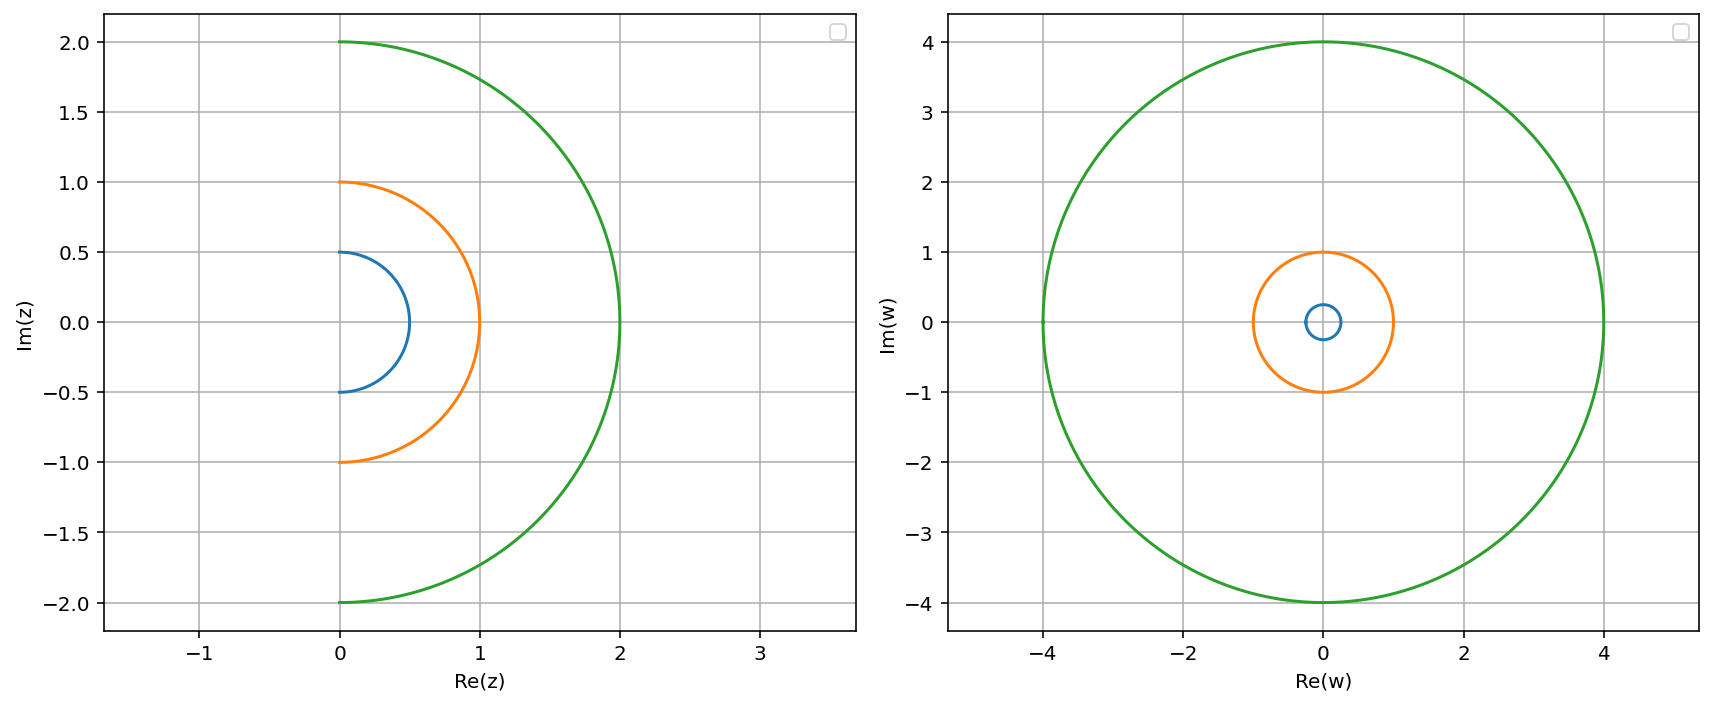
\includegraphics[scale=0.4]{images/2026-03-23-complex_02.png}
\end{figure}


\paragraph{Mapping $1/z$.} This mapping can be rewritten

\be\label{2026-03-23:eq1}
w = \frac{1}{z} = \frac{\bar{z}}{|z|^2}
\ee

This is a reflection on the real axis (due to the conjugate operation) and a scaling by $1 / |z|^2$. So points outside the unit circle will be moved inside the unit circle and vice versa.

Lines on the real and imaginary axis are mapped into lines again. This is shown in the plot below.

\begin{figure}[H]
\centering
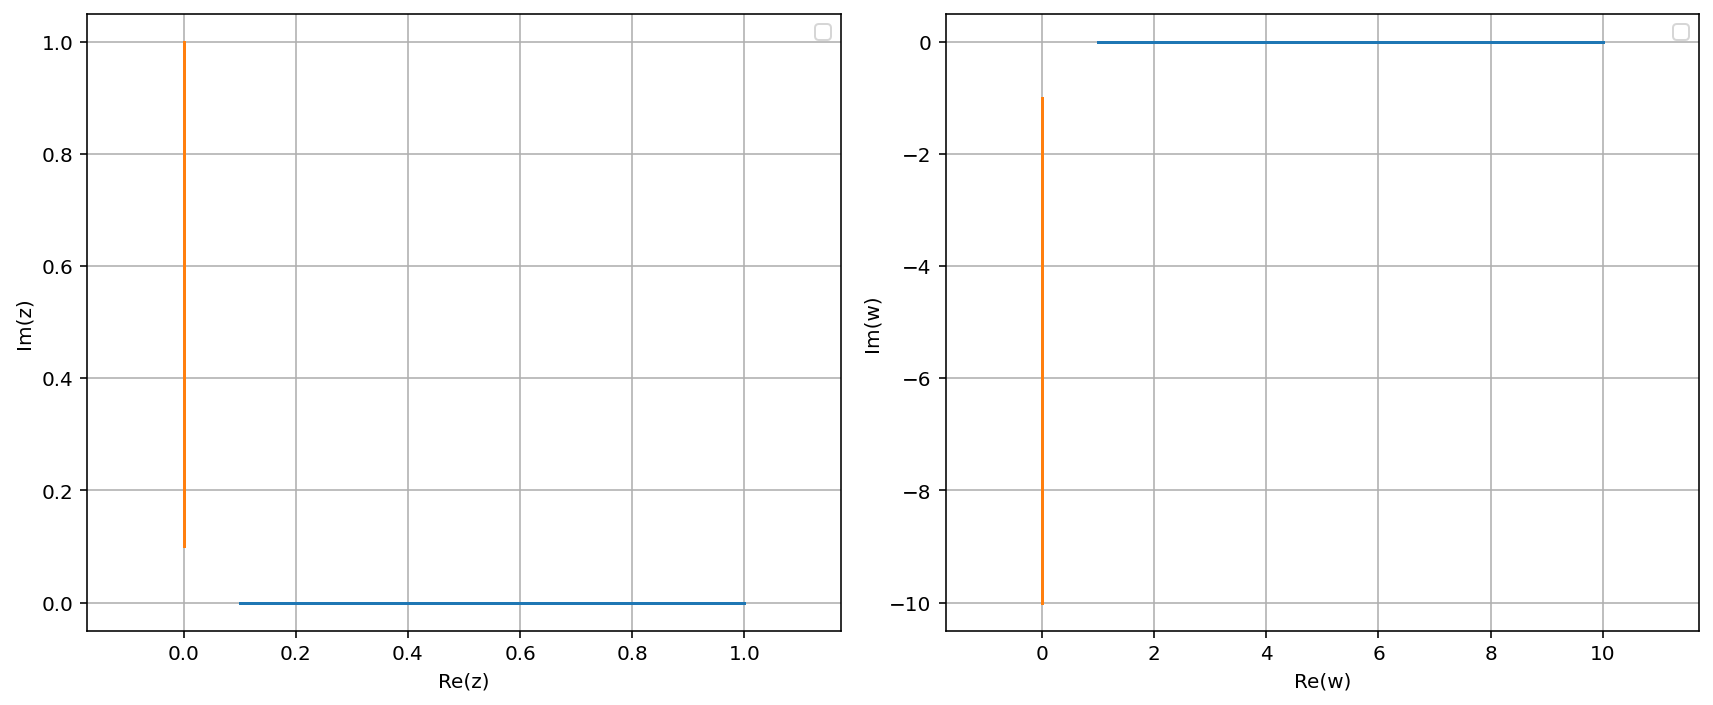
\includegraphics[scale=0.4]{images/2026-03-23-complex_10.png}
\end{figure}

Arbitrary lines are mapped onto circle.

\begin{figure}[H]
\centering
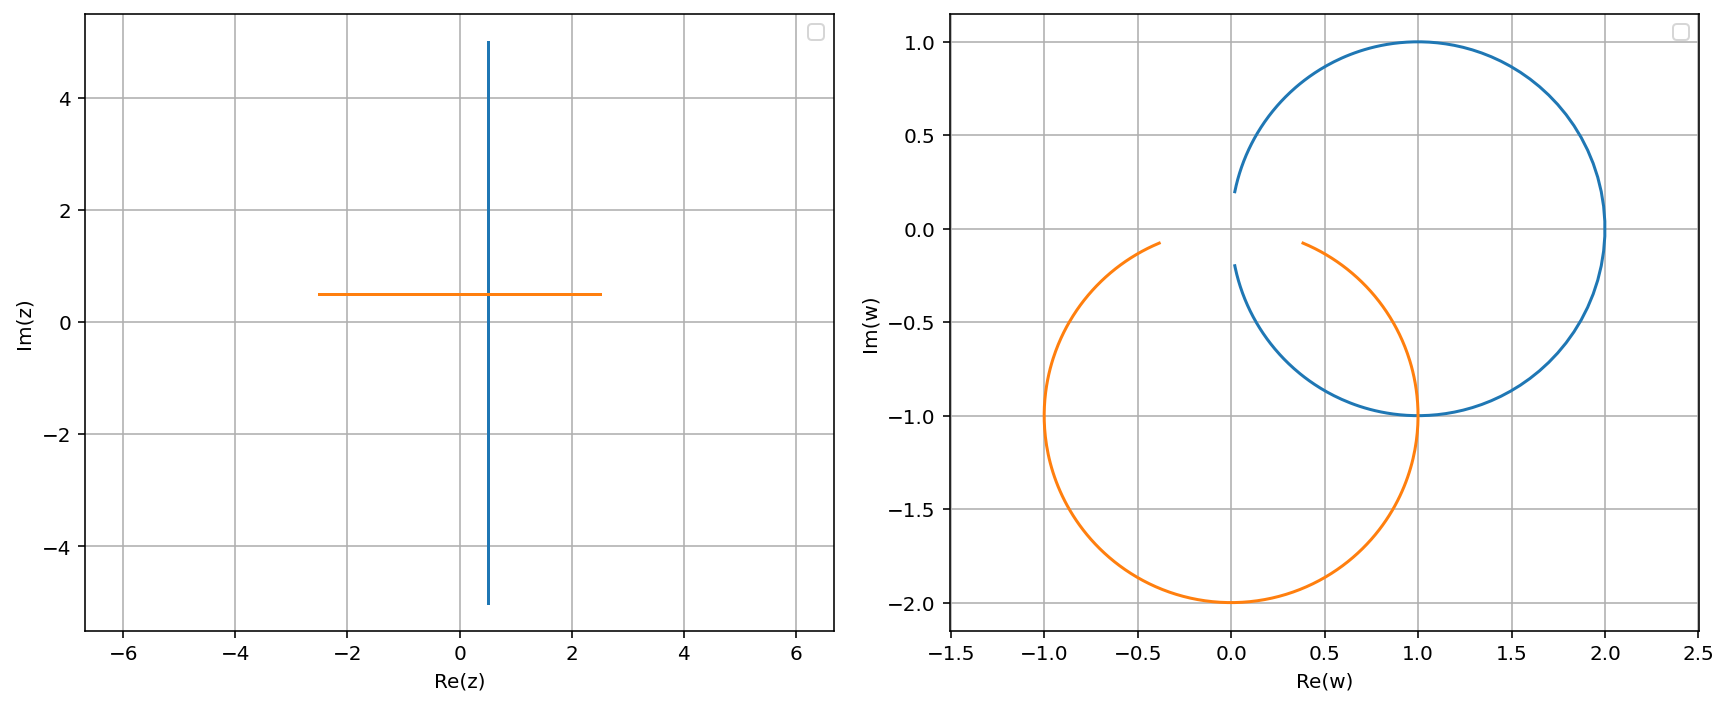
\includegraphics[scale=0.4]{images/2026-03-23-complex_11.png}
\end{figure}

And finally, circles are mapped onto circles; interestingly, not only circle with center at the origin, but circle with \emph{any} center point.

\begin{figure}[H]
\centering
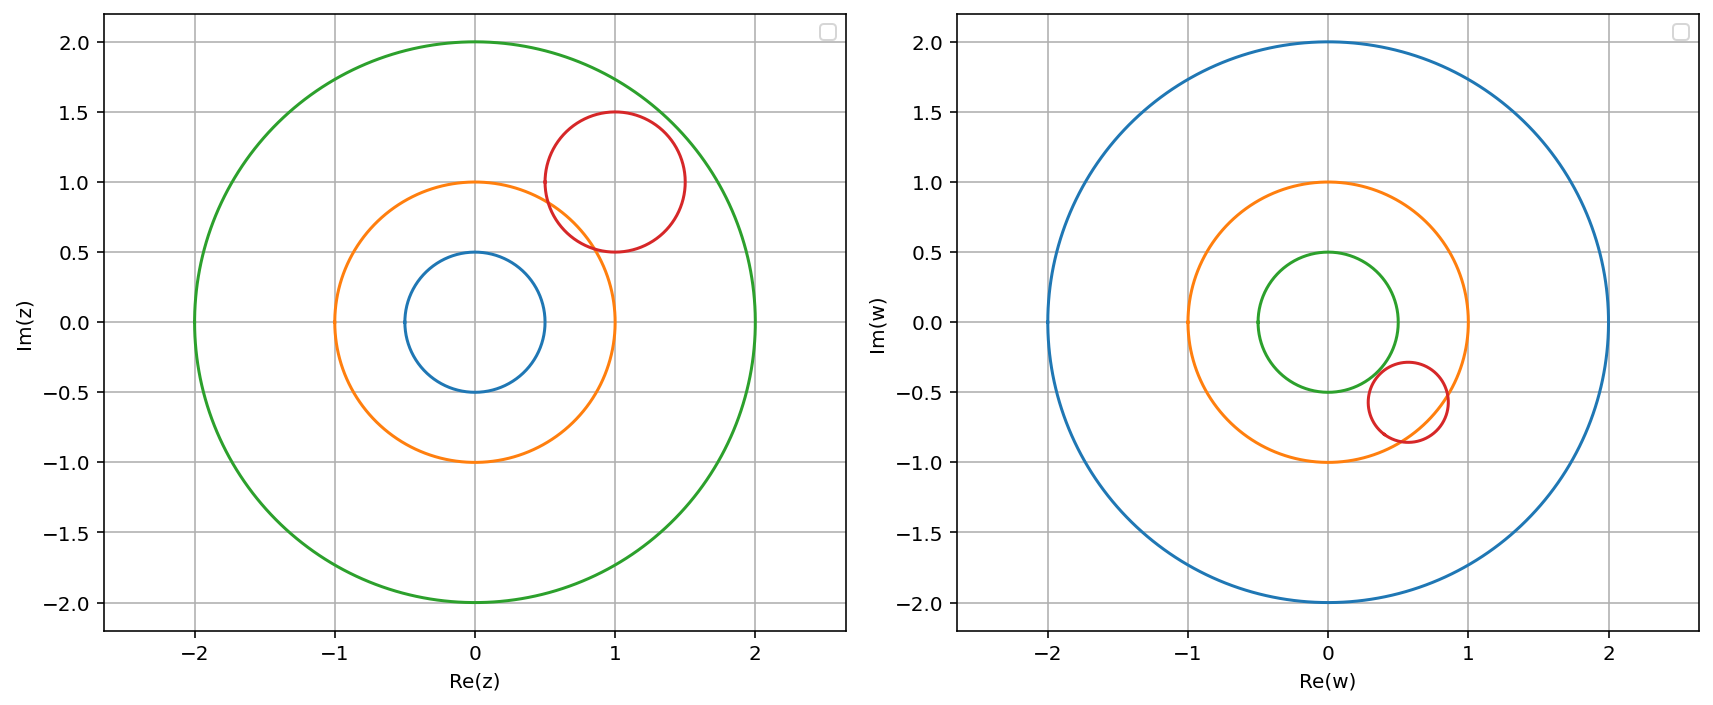
\includegraphics[scale=0.4]{images/2026-03-23-complex_12.png}
\end{figure}


To see the effect of the mapping, we start with equation of a circle with radius $r$ and center point $c$,

\bee
|z - c| = r
\eee

Substituing $z = 1/w$, we obtain

\bee
\left| \frac{1}{w} - c \right| = r \rightarrow |\frac{1 - wc}{w}| = r \rightarrow |1 - wc| = r |w|
\eee

We can square both sides; expanding the RHS yields

\bee
(1 - wc)(1 + \bar{wc}) = r^2 |w|^2 \rightarrow 1 - wc - \bar{wc} + |c|^2 |w|^2 = r^2 |w|^2 \rightarrow 1 - wc - \bar{wc} + |w|^2 (|c|^2 - r^2) = 0
\eee

We rearrange terms

\bee
|w|^2 - \frac{wc + \bar{wc}}{|c|^2 - r^2} + \frac{1}{|c|^2 - r^2} = 0 \rightarrow |w|^2 - \frac{wc + \bar{wc}}{|c|^2 - r^2} = - \frac{1}{|c|^2 - r^2} 
\eee

We now complete the square to obain a quadratic expression in $w$,

\bee
\left| w - \frac{\bar{c}}{|c|^2 - r^2}\right|^2 = \frac{|c|^2}{(|c|^2 - r^2)^2} - \frac{1}{|c|^2 - r^2} = \frac{|c|^2 - |c|^2 + r^2}{(|c|^2 - r^2)^2} = \frac{r^2}{(|c|^2 - r^2)^2}
\eee

From this we see that this is a circle with center point $\frac{\bar{c}}{|c|^2 - r^2}$ and radius $\frac{r}{(|c|^2 - r^2)}$.


\paragraph{Different Calculation - does not work yet}



We can make this more clear by expanding \eqref{2026-03-23:eq1},

\bee
w = u + jv = \frac{1}{z} = \frac{\bar{z}}{|z|^2} = \frac{x - jy}{x^2 + y^2}
\eee

From this follows the expression for $w = u + jv$,

\be\label{2026-03-23:eq2}
u = \frac{x}{x^2 + y^2} = \frac{x}{r}, \quad v = \frac{-y}{x^2 + y^2} = - \frac{y}{r}
\ee

with $r = x^2 + y^2$. 






We can represent a general circle using four real numbers $A, B, C, D$ with

\bee
B^2 + C^2 > 4AD
\eee

Then

\bee
A(x^2 + y^2) + Bx + Cy + D = 0
\eee

represents an arbitrary circle ($A \neq 0$) or a line ($A = 0$). We can rearrange this to express the circle center and radius more clearly; in fact, we have

\bee
\left( x + \frac{B}{2A}\right)^2 + \left( y + \frac{C}{2A}\right)^2 = \left( \frac{\sqrt{B^2 + C^2 - 4 AD}}{2A}\right)^2
\eee

We rewrite \eqref{2026-03-23:eq2} as

\bee
x = ur, \quad y = -vr
\eee

Substituing these back into $r = x^2 + y^2$ yields $r = r^2 (u^2 + v^2) \rightarrow r = \frac{1}{u^2 + v^2}$. Now we substitute back into the original circle equation,

\begin{align*}
A(x^2 + y^2) + Bx + Cy + D &= A r + B ur - C vr  + D \\ 
&= A \frac{1}{u^2 + v^2} + B \frac{u}{u^2 + v^2} +C \frac{-v}{u^2 + v^2} + D = 0    
\end{align*}

Multiplyig with $u^2 + v^2$ finally yields

\bee
D (u^2 + v^2) + B u - C v + A = 0
\eee

and this is again a circle equation.

%%% Local Variables:
%%% mode: latex
%%% TeX-master: "journal"
%%% End:
